\subsection{\bt{End-to-End Feature Reuse on RelBench}{RelBench 上的端到端特征复用}}
\label{sec:relbench-eval}
\bi{Reusing validated features reduces repeated exploration during retraining while preserving predictive quality across all six RelBench tasks. From the second cutoff onward, \system\ uses \RbStackMavraTokSave\% fewer tokens on rel-stack and \RbTrialMavraTokSave\% fewer on rel-trial than agents without memory.}
{复用已验证特征减少了重训时的重复探索，同时在 RelBench 的全部六项任务上保持预测质量。从第二个截点起，\system\ 相对无记忆智能体在 rel-stack 上少用 \RbStackMavraTokSave\% 的 token，在 rel-trial 上少用 \RbTrialMavraTokSave\%。}
\bi{\emph{Benchmark and timeline.} Periodic retraining lets us observe reuse as both tasks and data evolve. We use RelBench's task definitions and metrics on two databases~\cite{robinson2024relbench}. The seven-table rel-stack database supports user-engagement, user-badge, and post-votes; the fifteen-table rel-trial database supports study-outcome, study-adverse, and site-success. Each task has an agent that starts a new session at each of five cutoffs, while rows from the next period are appended between cutoffs. Memory can therefore transfer across successive sessions of one task and across agents working on different tasks.}
{\emph{基准与时间线。}定期重训使我们能够观察任务与数据演进过程中的复用。我们在 RelBench 的两个数据库上采用其原有任务定义和指标~\cite{robinson2024relbench}。含七张表的 rel-stack 提供 user-engagement、user-badge 和 post-votes 三项任务；含十五张表的 rel-trial 提供 study-outcome、study-adverse 和 site-success。每项任务由一个智能体负责，在五个截点各开始一次新会话，截点之间追加下一期数据。因此，记忆既可服务同一任务的后续会话，也可在负责不同任务的智能体之间传递。}

\bi{The last cutoff is RelBench's official split. Each preceding cutoff moves back by one task window, and RelBench's code regenerates the labels; at the last cutoff, these match the official tables row by row.}
{最后一个截点采用 RelBench 官方划分，此前每个截点依次前移一个任务窗口。标签由 RelBench 代码重新生成，最后一个截点的标签与官方表逐行一致。}
\bi{\emph{Sessions.} The no-memory and four memory arms share the same \llmmodel{} agent, using DeepSeek's API in thinking mode with low effort. Memory operations use the same model under each method's documented inference settings. The common tools expose schema and joins, read-only SQL, \code{validate\_features}, and \code{submit}. Feature SQL returns one row per seed using data dated at or before seed time, with a 600\,s execution limit. Validation trains a fixed LightGBM~\cite{ke2017lightgbm} on a 50,000-seed sample and returns its validation score.}
{\emph{会话。}无记忆组与四个记忆方法共用同一个 \llmmodel{} 智能体，通过 DeepSeek API 运行思考模式，推理强度为低。记忆操作使用同一模型，采用各方法复现说明中的推理设置。共用工具提供模式与连接查询、只读 SQL、\code{validate\_features} 和 \code{submit}。特征 SQL 使用不晚于种子时间的数据，每个种子返回一行，执行限时 600 秒；验证在 50,000 个种子的样本上训练固定 LightGBM~\cite{ke2017lightgbm}，并返回验证分数。}

\bi{A session has a budget of 40 LLM calls and 8 validations, and stops after two consecutive validations without improvement. From the second cutoff onward, refitting the previous cutoff's model on new data sets a validation target. Reaching it leaves one further improvement attempt within five LLM calls. Each validation is audited on 5,000 seeds by hiding later rows and recomputing features. Leaking validations are excluded and leaking submissions refused; test labels remain hidden from agents and memories. Sessions without a valid solution receive the entity-table reference score.}
{每个会话最多进行 40 次大模型调用和 8 次验证，连续两次验证未提升也会停止。从第二个截点起，将前一截点模型在新数据上重训，所得验证分数作为目标；达到目标后，还可在五次大模型调用内尝试一次改进。每次验证都在 5,000 个种子上隐藏更晚的行、重算特征，以审计泄漏。泄漏的验证不计分，泄漏的提交被拒绝；智能体和记忆始终看不到测试标签。未得到有效方案的会话按实体表参照计分。}
\bi{\emph{Baselines.} Five published methods cover agent memory and task-specific data preparation. ACE maintains a playbook per agent, updated after each session by its official reflector and curator without ground truth~\cite{zhang2026ace}. G-Memory uses its official implementation to share one memory across a database's agents~\cite{zhang2025gmemory}. AWM maintains a workflow memory per agent, using the official prompt to reinduce workflows from successful sessions after each session~\cite{wang2025awm}. The no-memory baseline uses the same agent with memory disabled.}
{\emph{基线。}五个已发表方法覆盖智能体记忆和针对单项任务的数据准备。ACE 为每个智能体维护一本手册，每次会话后由官方的反思者和整理者在无真实标签的设置下更新~\cite{zhang2026ace}。G-Memory 使用官方实现，让一个数据库的智能体共享一份记忆~\cite{zhang2025gmemory}。AWM 为每个智能体维护工作流记忆，每次会话后用官方提示词从成功会话重新归纳工作流~\cite{wang2025awm}。无记忆基线使用同一个智能体，但关闭记忆。}

\bi{DeepPrep and FeatPilot search afresh for each task. DeepPrep's official LLM agent explores operator pipelines as a tree with execution feedback~\cite{fan2026deepprep}. We retain its reasoning loop, prompts, operators, and executor, using the study's model on the task's tables. It explores on 2,000 seeds, then runs its solution on all seeds with the same 600\,s limit per split. FeatPilot searches join paths for useful features without an LLM~\cite{liang2025featpilot}; our implementation follows the paper and bounds every aggregate by seed time. All methods requiring a success signal use a validation score above the entity-table reference. The artifact provides configurations and reproduction instructions.}
{DeepPrep 与 FeatPilot 对每项任务重新搜索。DeepPrep 的官方 LLM 智能体在执行反馈下以树结构探索算子流水线~\cite{fan2026deepprep}；我们保留其推理循环、提示词、算子和执行器，在任务表上使用本研究的模型。它先在 2,000 个种子上探索，再将方案用于全部种子，每个划分同样限时 600 秒。FeatPilot 不用 LLM，通过搜索连接路径获得有用特征~\cite{liang2025featpilot}；我们的实现遵循论文，并将每个聚合限制在种子时间以内。需要成功信号的方法统一使用高于实体表参照的验证分数。配置与复现步骤见工件。}
\bi{\emph{The workload.} Without memory, a session takes a median of \RbNoneMedLlm\ LLM calls and \RbNoneMedTok\,k tokens, \RbSchemaProbe\% of its tool calls inspect the schema or probe values, and \RbSchemaRepeat\% of the schema calls in later sessions repeat a call that an earlier session on the same database already made.}
{\emph{工作负载。} 没有记忆时，一个会话的 LLM 调用中位数为 \RbNoneMedLlm\ 次、token 中位数为 \RbNoneMedTok\,k，\RbSchemaProbe\% 的工具调用在看结构或探查取值，后续会话里 \RbSchemaRepeat\% 的看结构调用重复了同一数据库上更早会话已做过的调用。}

\begin{table*}[t]
\caption{\bt{RelBench: predictive quality, valid solutions, and reuse cost. Each method runs three tasks at five cutoffs per database.}{RelBench：预测质量、有效方案与复用代价。每种方法在每个数据库上运行三个任务、五个截点。}}
\label{tab:relbench}
\centering
\ifbilingual\footnotesize\else\small\fi
\setlength{\tabcolsep}{2.8pt}
\renewcommand{\arraystretch}{1.08}
\newcommand{\RbPanelHeader}[4]{%
  \multicolumn{12}{@{}l}{\textbf{#1}}\\[2pt]
  & \multicolumn{6}{c}{\bh{Reuse cost: cutoffs 2--5}{复用代价：截点 2--5}}
  & \multicolumn{3}{c}{\bh{Mean test score: cutoffs 1--5}{平均测试分数：截点 1--5}}
  & \multicolumn{2}{c}{\bh{Quality summary}{质量汇总}}\\
  \cmidrule(lr){2-7}\cmidrule(lr){8-10}\cmidrule(l){11-12}
  \bh{Method}{方法} & \bh{Tokens\\(M)}{token\\（百万）} & \bh{Token\\ratio}{token\\比率}
  & \bh{LLM\\calls}{LLM\\调用} & \bh{Tool\\calls}{工具\\调用}
  & \bh{Obs.\\min}{观测\\分钟} & \bh{Cost\\(USD)}{美元}
  & #2 & #3 & #4 & \bh{Valid\\sessions}{有效会话} & \bh{Quality\\tasks}{达标任务}\\
  \midrule
}
\begin{tabular*}{\textwidth}{@{\extracolsep{\fill}}lrrrrrrrrrcc@{}}
\toprule
\RbTableBody
\bottomrule
\end{tabular*}
\par\smallskip
\parbox{\textwidth}{\footnotesize\raggedright
\bt{Cost columns total 12 sessions at cutoffs 2--5, including memory operations; token ratios are relative to no memory. Test scores average all five cutoffs, using the entity-table reference for sessions without a valid solution. \emph{Valid sessions}: non-fallback solutions (/15). \emph{Quality tasks}: tasks retaining no-memory predictive quality (/3), with $\mathrm{AUC}\geq\mathrm{AUC}_0-0.01$ or $\mathrm{MAE}\leq 1.02\,\mathrm{MAE}_0$. Subscript 0 denotes no memory; best task means are bold. Time and USD accounting are specified in Section~\ref{sec:relbench-eval}.}{代价列合计截点 2--5 的 12 个会话，含记忆操作；token 比率以无记忆为参照。测试分数取五个截点的平均，无有效方案的会话采用实体表参照分数。有效会话计数排除参照回退（共 15 个）；达标任务指保持无记忆预测质量的任务数（共 3 项），满足 $\mathrm{AUC}\geq\mathrm{AUC}_0-0.01$ 或 $\mathrm{MAE}\leq 1.02\,\mathrm{MAE}_0$。下标 0 表示无记忆；各任务最佳平均分加粗。时间与美元计量见第~\ref{sec:relbench-eval} 节。}
}
\end{table*}

\begin{figure}[t]
\centering
% Vector drawing generated by tools/figures/relbench_cumulative.py from exp/2026-10-20-relbench/paper-sessions.json; rerun it after the numbers change.
\ifbilingual
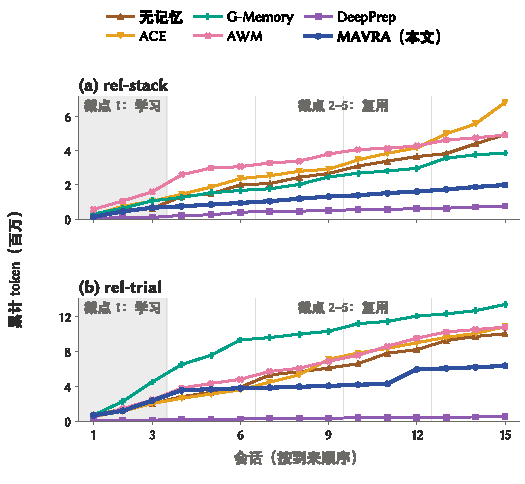
\includegraphics[width=\linewidth]{figures/relbench-cumulative-zh}
\else
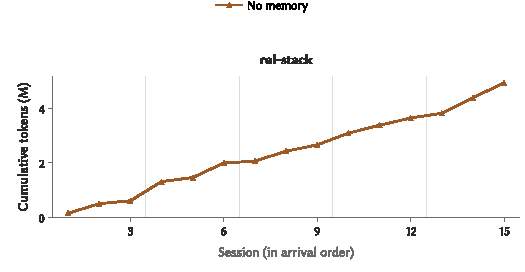
\includegraphics[width=\linewidth]{figures/relbench-cumulative}
\fi
\caption{\bt{Cumulative tokens of the RelBench sessions in arrival order, memory operations included; thin rules separate the five cutoffs. After the first cutoff, \system's agents start from the verified task program and its curve flattens, while the other methods keep paying for exploration at every cutoff.}{按到来顺序累计的 RelBench 会话 token（含记忆操作）；细线分隔 5 个截点。第一个截点之后，\system\ 的智能体从经验证的任务方案出发，曲线变平；其他方法在每个截点都继续为探索付费。}}
\label{fig:relbench-cumulative}
\Description{Two line charts, rel-stack and rel-trial, of cumulative tokens in millions against the session index from 1 to 15, one line per method.}
\end{figure}

\bi{\emph{Results.} Table~\ref{tab:relbench} shows that lower reuse cost is accompanied by comparable predictive quality. All six tasks meet the evaluation criteria: \RbStackMavraNotWorse/3 on rel-stack and \RbTrialMavraNotWorse/3 on rel-trial have $\mathrm{AUC}\geq\mathrm{AUC}_0-0.01$ or $\mathrm{MAE}\leq1.02\,\mathrm{MAE}_0$, where subscript 0 denotes no memory. From the second cutoff onward, \system\ also uses \RbStackMavraVsBest\% fewer tokens on rel-stack and \RbTrialMavraVsBest\% fewer on rel-trial than the most token-efficient agent-memory baseline. Figure~\ref{fig:relbench-cumulative} traces how these savings accumulate. Including the first cutoff, when agents explore and build memory, total token reductions relative to no memory remain \RbStackMavraTokSaveAll\% and \RbTrialMavraTokSaveAll\%.}
{\emph{结果。}表~\ref{tab:relbench} 表明，复用代价下降的同时，预测质量保持相当。六项任务均满足评估标准：rel-stack 的 \RbStackMavraNotWorse/3 项和 rel-trial 的 \RbTrialMavraNotWorse/3 项达到 $\mathrm{AUC}\geq\mathrm{AUC}_0-0.01$ 或 $\mathrm{MAE}\leq1.02\,\mathrm{MAE}_0$，下标 0 表示无记忆基线。从第二个截点起，\system\ 相对最省 token 的智能体记忆方法，在 rel-stack 上进一步减少 \RbStackMavraVsBest\%，在 rel-trial 上减少 \RbTrialMavraVsBest\%。图~\ref{fig:relbench-cumulative} 展示这些节省如何累积。将智能体探索并建立记忆的首截点也计入后，相对无记忆的总 token 降幅仍为 \RbStackMavraTokSaveAll\% 和 \RbTrialMavraTokSaveAll\%。}

\bi{The monetary saving is smaller because reuse changes the token mix. On rel-stack, cached input falls from 86\% to 67\% of tokens while output rises from 11\% to 15\%. Much of the avoided volume is therefore inexpensive cached input.}
{金额降幅较小，是因为复用改变了 token 构成。rel-stack 上，缓存命中输入的占比从 86\% 降至 67\%，输出占比从 11\% 升至 15\%；省去的用量有很大一部分是价格较低的缓存命中输入。}
\bi{\emph{Session outcomes and measurement.} DeepPrep produces no valid solution in \RbStackDeepPrepUnsolved/15 sessions on rel-stack and \RbTrialDeepPrepUnsolved/15 on rel-trial; these receive the reference score. Eleven failures occur when executing the final pipeline on the full seed split exceeds 600\,s (five on rel-stack, six on rel-trial); two rel-stack searches terminate after exceeding the official five-error limit. FeatPilot completes all sessions without LLM calls. The evaluation comprises 210 sessions: seven methods, two databases, and one five-cutoff sequence with three tasks per cutoff. Token volume and LLM/tool call counts are the primary efficiency measures. Table~\ref{tab:relbench} also reports end-to-end wall-clock durations (which include external LLM API latency); full execution and measurement details are documented in the artifact.}
{\emph{会话结果与测量。}DeepPrep 在 rel-stack 的 15 个会话中有 \RbStackDeepPrepUnsolved\ 个、在 rel-trial 中有 \RbTrialDeepPrepUnsolved\ 个没有有效方案，按参照计分。11 次失败是最终流水线在完整种子划分上执行超过 600 秒（rel-stack 5 次、rel-trial 6 次）；另 2 次 rel-stack 搜索因超过官方的五次报错上限而终止。FeatPilot 完成全部会话且不调用 LLM。评估共包含 210 个会话：7 个方法在 2 个数据库上各运行一条五截点序列，每个截点 3 个任务。主要效率指标为 token 用量及 LLM／工具调用数。表~\ref{tab:relbench} 同时报告端到端墙钟耗时（包含外部 LLM API 延迟）；完整的执行与测量细节见工件。}

\bi{\emph{Where the savings come from.} A \system\ agent begins with its task's validated program and compiled entity-level feature definitions from earlier sessions. The program provides executable SQL, and the definitions support feature selection and refinement. Together they usually let the agent reach its target at the first validation, leaving the remaining budget for focused improvement. The measured savings therefore describe this combined reuse path.}
{\emph{节省的来源。}\system\ 的智能体从本任务已验证的方案和此前会话提供的实体级特征定义开始。方案提供可执行 SQL，定义支持进一步选择和调整特征。二者结合，通常使智能体在第一次验证时达到目标，把剩余预算用于有针对性的改进。因此，这里的节省对应两者共同构成的复用路径。}

\bi{The reduction in exploration is visible in tool use. From the second cutoff onward, \system\ makes \RbStackMavraExplore\ schema and probe calls per session on rel-stack, compared with \RbStackNoneExplore\ without memory. ACE, AWM, and G-Memory make \RbStackACEExplore, \RbStackAWMExplore, and \RbStackGMemExplore\ such calls: their playbooks, workflows, and trajectories still require the agent to inspect tables and turn prior knowledge into SQL. DeepPrep and FeatPilot restart that search for each task and cutoff.}
{工具调用反映了探索量的下降。从第二个截点起，\system\ 在 rel-stack 上每会话进行 \RbStackMavraExplore\ 次模式与取值探查，无记忆为 \RbStackNoneExplore\ 次。ACE、AWM 和 G-Memory 分别进行 \RbStackACEExplore、\RbStackAWMExplore\ 和 \RbStackGMemExplore\ 次：它们提供的手册、工作流与轨迹仍需要智能体查看表，并将已有知识转成 SQL。DeepPrep 和 FeatPilot 则在每项任务、每个截点重新开始搜索。}
